\newpage

\subsection{Décodeur 7seg}

\begin{figure}[ht]
    \centering
    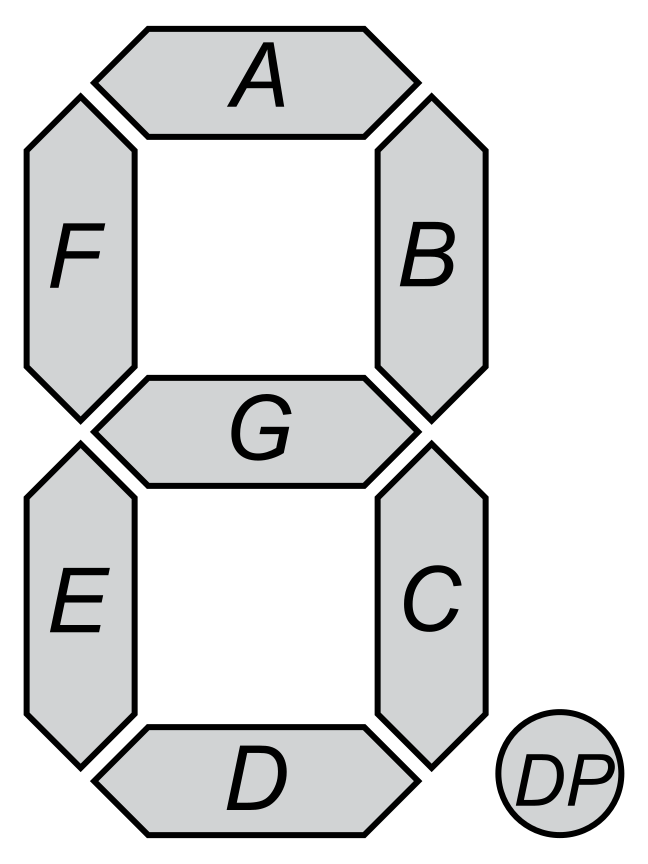
\includegraphics[scale = 0.1]{img/SevenSegDisplay.png}
    \caption{Segments d'un afficheur}
    \label{fig:seven_segment_display}
\end{figure}

Un afficheur sept segments est utilisé pour afficher des informations vers un utilisateur en allumant une partie des segments. Par exemple, pour afficher le chiffre \textit{2}, on allume les segments \textit{A, B, D, E, G}.

\medskip

- On veut afficher sur l'afficheur sept segments, les chiffres allant de $0_h$ à $F_h$. Combien de bits il faut en entrée et en sortie pour pouvoir représenter ces chiffres.

\medskip

- Dessiner sur une feuille l'entité du décodeur sept segments en faisant apparaître l'entrée \textit{x} qu'on veut decoder et la sortie \textit{y} qui contient les segments qu'on veut allumer et éteindre en fonction l'entrée \textit{x}. Faire apparaître les entrées/sorties vectorisées.

\medskip

- Décrire la table de vérité de l'afficheur sept segments pour les chiffres allant de \textbf{$0_h$ à $F_h$} à l'aide de l'entité que vous avez dessiné précédemment et de la figure \ref{fig:seven_segment_display}.

\medskip

- Décrire l'entité \textbf{seven\_segment} et l'architecture \textbf{rtl\_seven\_segment} de votre table de vérité en VHDL.

\medskip

- Simuler et vérifier le bon comportement de votre table de vérité.

\medskip

- Connecter les entrées de votre décodeur sept segments aux switchs (SW$x$) et les sorties aux afficheurs sept segments (HEX$x$) de la carte DE2. Tester et vérifier le bon fonctionnement.

\medskip

- Expliquer pourquoi les bons segments sont éteints? Instancier le composant \textit{seven\_segment} à un module top level ou faire les modifications nécessaires au composant \textit{seven\_segment} pour que les bons segments s'allument.
